\chapter{Value At Risk}
\label{var-and-credit-risk}

\section{VaR}
\label{value-at-risk}

The \emph{Value at Risk} (VaR) of a portfolio is usually used when it is important to know to a certain confidence level how much will be the maximum loss in the next $N$ days (time horizon). It can be interpreted as the loss level over $N$ days that has a probability of only \((100 - X)\%\) of being exceeded. By definition it is a function of two parameters: the time horizon and the confidence level. 

Mathematically the VaR is the loss corresponding to the \((100-X)\textrm{th}\) percentile of the portfolio change in value distribution over the next $N$ days (e.g. in Figure~\ref{fig:var_loss} the graphical representation of the VaR assuming a normal distribution for the changes in value is shown, with $N=1$ and $X=95$).

\begin{figure}[htb]
\centering
  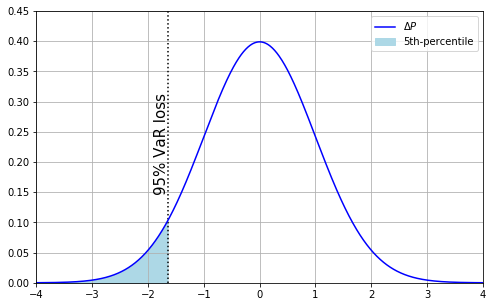
\includegraphics[width=0.6\linewidth]{figures/95_var.png}
  \caption{Example of 95\% VaR on the distribution of changes in value.}
  \label{fig:var_loss}
\end{figure}
    
VaR is useful to summarize all the information about the risk of a portfolio in one single number, but this can also be considered its main limitation as it implies too much simplification of such a complex task.

Concerning the time horizon parameter it is usually set to $N=1$ since it is not easy to estimate market variables over periods longer than one day. Nevertheless to generalize the VaR estimate it is assumed

\begin{equation}
\textrm{N-day VaR} = \textrm{1-day VaR}\cdot \sqrt{N}
\label{eq:var_horizon}
\end{equation}
This relation is true only if the portfolio changes in value over the considered period of time have independent and identical normal distributions with zero mean, otherwise it is just an approximation.

In the next Section the methods that can be used to estimate the VaR
will be reviewed.

\section{How to Estimate the VaR}
\label{how-to-estimate-the-var}

In the proposed examples historical series of Apple and Netflix are used also it has been assumed to have a portfolio made of \textbf{60\% of AAPL and 40\% NFLX stocks}.
 
You can download the dateset with \texttt{yfinance} as in the following code or to check out \href{https://raw.githubusercontent.com/matteosan1/finance_course/develop/libro/input_files/historical_data.csv}{historical\_data.csv}.

\begin{ipython}
import yfinance as yf
	
proxy = yf.Tickers(['AAPL', 'NFLX'])
df = proxy.history(start='2014-01-02', end='2021-03-27')['Close']
print (df.head())
\end{ipython}
\begin{ioutput}
                 aapl       nflx
Date
2014-01-02  17.598297  51.831429
2014-01-03  17.211735  51.871429
2014-01-06  17.305593  51.367142
2014-01-07  17.181829  48.500000
2014-01-08  17.290642  48.712856
\end{ioutput}
\noindent
In the following we are going to add a new column with the daily return to the dataframe.

\begin{ipython}
import pandas as pd
import numpy as np

w = np.array([0.6, 0.4])
df['AAPL_rets'] = df['AAPL'].pct_change()
df['NFLX_rets'] = df['NFLX'].pct_change()

print (df.head())
\end{ipython}
\begin{ioutput}
                 AAPL       NFLX  AAPL_rets  NFLX_rets
Date                                                  
2014-01-02  17.542171  51.831429        NaN        NaN
2014-01-03  17.156841  51.871429  -0.021966   0.000772
2014-01-06  17.250401  51.367142   0.005453  -0.009722
2014-01-07  17.127035  48.500000  -0.007151  -0.055817
2014-01-08  17.235500  48.712856   0.006333   0.004389
\end{ioutput}

\subsection{Historical Simulation}
\label{historical-simulation}

In order to estimate the VaR from historical series, we need to collect the market variables "affecting" the portfolio over the last $N$ days (with $N$ quite large).

The variation over each day in our time interval will provide different scenarios to be applied to today's market values. In each "simulation" the historical variation is applied and the distribution of portfolio change in value (\(\Delta P\)) is computed. The VaR estimate will be the $(100 - X)\%$ percentile of this distribution. 

Clearly such kind of simulation heavily relies on the assumption that past behaviors are indicative of what might happen in the future, that's why it is important that out historical series was as large as possible.

Mathematically the evolution of the portfolio can be simulated by rescaling the market variables (e.g. \(x_1(t), x_2(t)\)) according to their variations between day \(i\) and \(i-1\)

\begin{equation}
P_i(t_n+1) = P\left(x_1(t_n)\cfrac{(x_1(t_i)-x_1(t_{i-1}))}{x_1(t_{i-1})}, x_2(t_n)\cfrac{(x_2(t_i)-x_2(t_{i-1}))}{x_2(t_{i-1})}\right)
\end{equation}

At each simulation the portfolio value $P_i$ is determined by the \emph{scalar product} between the invested amount (the weights $w_i$) and the price of each portfolio component ($p_i$), i.e. $\sum_{i} w_i \cdot p_i$. In \texttt{python} it is indicated with the method \texttt{.dot}. For more information about scalar product, vector and matrices see Chapter~\ref{sec:matrices}.

Finally the distribution of possible changes in the portfolio value \(P_i\) is drawn and the VaR computed by taking the appropriate percentile.
Figure~\ref{fig:hist_var} shows the resulting VaR. 

\begin{ipython}
import numpy as np

rets = []
for idx in df.index[1:]:
rets.append(w[0]*df.loc[idx]['AAPL_rets'] + w[1]*df.loc[idx]['NFLX_rets'])

price = [df.iloc[-1]['AAPL'], df.iloc[-1]['NFLX']]
portfolio_price = w.dot(price)
hist_var = portfolio_price*np.percentile(rets, 1)

print ('Historical VAR is {:.3f}'.format(hist_var))
\end{ipython}
\begin{ioutput}
Historical VAR is -12.996
\end{ioutput}

\begin{figure}[htb]
\centering
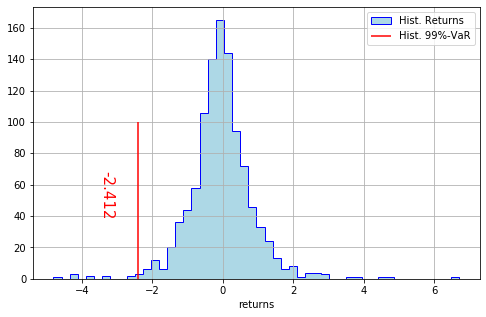
\includegraphics[width=0.7\textwidth]{figures/historical_var}
\caption{Distribution of the changes of values estimated from historical data. The red line shows the 99\% VaR.}
\label{fig:hist_var}
\end{figure}

\subsection{Model Approach}
\label{model-approach}

The portfolio $P$ consists of different amounts $w_i$ invested on two assets. If with $\Delta x_i$ we denote the daily return of the $i^{th}$ asset the portfolio change in value can be expressed as

\begin{equation}
\Delta P = \sum_{i=1}^n w_i \Delta x_i
\end{equation}

If we then assume that the asset variations are normally distributed with zero mean (in this approach is typical to assume the expected change in a market variable over the considered period equal to zero), \(\Delta P\) will be also normally distributed (as a sum of normal distribution) with zero mean.

To estimate the VaR we just need to compute the standard deviation of $\Delta P$. In the general case with many different assets, $\sigma_i$ indicates the daily volatility of the $i^{th}$ asset and $\rho_{ij}$ the correlation coefficient between the assets $i$ and $j$. The variance of $\Delta P$ can then be expressed as

\begin{align}
\begin{split}
\sigma^2_P & = \sum_{i=1}^{n}\sum_{j=1}^{n}\rho_{ij}w_i w_j \sigma_i \sigma_j \\
& = \sum_{i=1}^{n} w_i^2 \sigma_i^2 + 2 \sum_{i=1}^{n}\sum_{j<i}^{n}\rho_{ij}w_i w_j \sigma_i \sigma_j 
\end{split}
\end{align}
\noindent
If we are interested in a longer time horizon we can use Eq.~\ref{eq:var_horizon}.

Once we have the variance of \(\Delta P\) it is easy to determine the appropriate percentile using the equations described in Appendix~\ref{transformation-to-standard-normal}.

\subsection{Monte Carlo Simulation}
\label{monte-carlo-simulation}

A very useful alternative to previous approaches is using a Monte Carlo simulation to generate the probability distribution for the $\Delta P$. 

Imagine we need to compute the 1-day VaR for our example portfolio. The simulation can be done either generating random returns from a distribution with mean and standard deviation obtained from the historical data of each stock, or by simulating the evolution of all the portfolio market variables in one day.

Let's start from the first case, computing mean and standard deviation of each historical dataset. We will sample various simulated returns from a multivariate Gaussian with such means and variances. One useful aspect of this method is that in principle other distributions than Gaussian could be used. 

Once we have the distribution of returns the VaR can be computed as usual, the result is shown in Fig.~\ref{fig:mc1_var}.

\begin{ipython}
from scipy.stats import multivariate_normal

mean = [np.mean(df['AAPL_rets']), np.mean(df['NFLX_rets'])]
cov = np.cov(df['AAPL_rets'][1:], df['NFLX_rets'][1:])
mvnorm = multivariate_normal(mean=mean, cov=cov)
np.random.seed(1)
n_sims = 100000
sim_returns = mvnorm.rvs(n_sims)
p_returns = [w.dot(s) for s in sim_returns]
mc_var = portfolio_price * np.percentile(p_returns, 1)

print('Simulated VAR is {:.3f}'.format(mc_var))
\end{ipython}
\begin{ioutput}
Simulated VAR is -11.267
\end{ioutput}

\begin{figure}[htb]
\centering
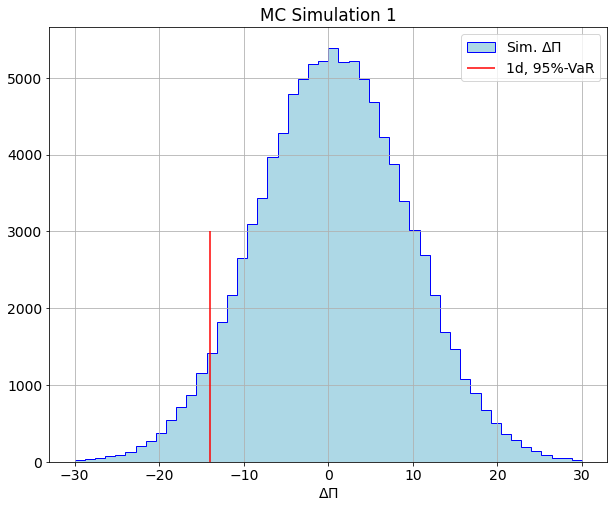
\includegraphics[width=0.7\textwidth]{figures/sim1_var}
\caption{Distribution of the changes of values estimated from simulated data. The red line shows the 99\% VaR.}
\label{fig:mc1_var}
\end{figure}

This result can be compared with VaR estimate determined by a simulation of the daily evolution of the stock price. We will use the log-normal evolution described in Section~\ref{derivation-of-log-normal-stochastic-differential-equation} where $\mu$ and $\sigma$ are the mean and variance estimated from the historical series. Figure~\ref{fig:mc2_var} shows the resulting distribution of the returns.

\begin{ipython}
from numpy.random import normal
from numpy import exp, sqrt

T = 1
trials = 100000
dP = []
for _ in range(trials):
    s = 0
    for i in range(2):
        s += w[i] * price[i] * exp((mean[i] - 0.5 * cov[i][i]) * T +
             sqrt(cov[i][i]) * sqrt(T) * normal())
    dP.append(portfolio_price - s)

mc_var2 = np.percentile(dP, 1)
print('Simulated VAR is {:.3f}'.format(mc_var2))
\end{ipython}
\begin{ioutput}
Simulated VAR is -13.717
\end{ioutput}

\begin{figure}[htb]
\centering
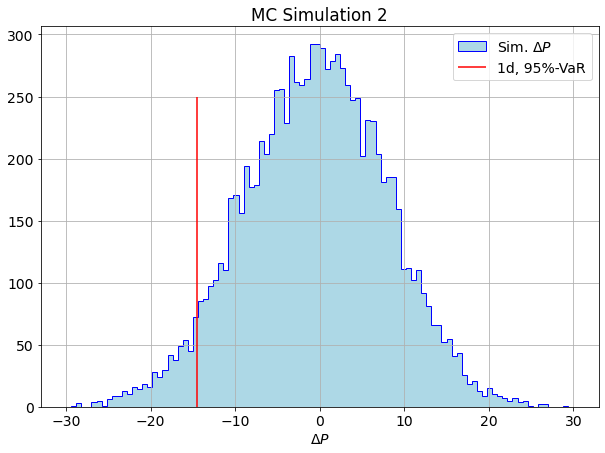
\includegraphics[width=0.7\textwidth]{figures/sim2_var}
\caption{Distribution of the changes of values estimated from simulation of the evolution of the stock prices. The red line shows the 99\% VaR.}
\label{fig:mc2_var}
\end{figure}

\subsection{Stress and Back Testing}
\label{stress-testing-and-back-testing}

In addition to calculating the value at risk of a portfolio, it is generally useful to check how it would behave under the most extreme market moves seen in the last years.

This kind of test is called \emph{stress test} and it is done by extracting from the historical series, particular days with exceptionally large variation of the market variables.
 
The idea is to take into account extreme events that can happen more frequently in reality than in a simulation (where usually Gaussian tails are assumed hence are quite small). For example a 5-standard deviation ($5\sigma$)move is expected to happen once every 7000 years but in practice can be observed twice over 10 years.

\begin{attention}
\subsubsection{$n\sigma$ Event Likelihood}
Such event has a probability to occur equal to $n\sigma$ so the occurrence frequency can be computed as 1 over $252\cdot\mathbb{P}(|x| \ge n\sigma$) (the 252 factor comes to the number of working days per year).

\begin{attpython}
from scipy.stats import norm

prob = norm.cdf(-5) * 2 # e.g. consider +- 5sigma movements
nyears = 1/prob/252
print (nyears)
\end{attpython}
\begin{ioutput}
6921.737673091067
\end{ioutput}
\noindent
So about seven thousand years as stated before.
\end{attention}

Another important check that could be done is the so-called \emph{back testing} which consists of checking how well the VaR estimate would have performed in the past. Basically it has to be tested how often the daily loss exceeded the N-days X\% VaR just computed. If it happens on about (100-X)\% of the times we can be confident that our estimate is correct.

\section{Credit VaR}
\label{credit-var-cr-var}

%exposure at any given future time is the
%larger between zero and the market value of the portfolio of derivative
%positions with a counterparty that would be lost if the counterparty
%were to default with zero recovery at that time.

\emph{Credit VaR} is defined in the usual way Value at Risk measures are (i.e. as percentile of a loss distribution).
In this case we are concerned with the default risk associated to one or multiple counter-parties in a specific portfolio instead of to the market risk.

To derive the loss distribution we need to consider the exposure $\textrm{EE}(\tau)$ defined as the sum of the discounted cash flows at the default date $\tau$. The corresponding loss is then given by

\begin{equation}
L_{\tau, \hat{T}} = (1 - R) \cdot \textrm{EE}(\tau)
\end{equation}
where \(\hat{T}\) is the risk horizon and $L$ is non-zero only in scenarios of early counter-party default. 

Given the above definitions we can express the Credit VaR as the X-quantile of $L_{\tau, \hat{T}}$.
With respect to the Value at Risk, the time horizon is usually set to one year and the percentile to $99.9^{th}$, so it returns the loss that is exceeded only in 1 case out of 1000. 

Credit VaR is actually either the difference of the percentile from the mean, or the percentile itself. There is more than one possible definition, anyway we  will use the latter.

%Consider your portfolio has a call option on equity with a final maturity of two years. To get the Credit-Var, roughly, you simulate the underlying equity up to one year, and obtain a number of scenarios for the underlying equity in one year. Also, you need to simulate the default scenarios up to one year, to know in each scenario whether the counter-parties have defaulted or not. 
%
%And then in each scenario at one year, if the counter-party
%has defaulted there will be a recovery value and all else will be lost.
%Otherwise, we price the call option over the remaining year using for
%example a Black Scholes formula. But this price is like taking the
%expected value of the call option payoff in two years, conditional on
%each scenario for the underlying equity in one year. Because this is
%pricing, this expected value will be taken under the pricing measure Q,
%not P. This gives the Black Scholes formula if the underlying equity
%follows a geometric brownian motion under Q.

\subsection{Credit VaR and MC Simulation}

Credit VaR can be calculated through a simulation of the basic financial variables underlying the portfolio up to the risk horizon; the simulation must of course include possible defaults of the counter-parties. 

In each simulation of the basic financial variables the portfolio is priced obtaining a number of scenarios to draw the loss distribution. It is then straightforward to derive the Credit VaR from it.

Consider a portfolio of twenty zero coupon bonds each one with a default probability of 8\% and the same face value (\euro{100}). The recovery rate in case of default is $R=40\%$ and the risk free rate is 1\%.

\begin{ipython}
import numpy as np
from datetime import date
from dateutil.relativedelta import relativedelta
from finmarkets import DiscountCurve, CreditCurve
from scipy.stats import uniform

bonds = 20
S = [1-0.08 for _ in range(bonds)]
FV = [100 for _ in range(20)]
R = 0.4
r = 0.01
obs_date = date.today()
pillars = [obs_date+relativedelta(years=i) for i in range(2)]
dfs = [1/(1+r)**i for i in range(2)]
dc = DiscountCurve(obs_date, pillars, dfs)
ccs = []
for i in range(bonds):
    ccs.append(CreditCurve(pillars, [1, S[i]]))
scenarios = 100000
losses = []
for _ in range(scenarios):
    loss = 0
    unif = uniform.rvs(size=bonds)
    for i in range(bonds):
        if unif[i] > ccs[i].ndp(pillars[-1]):
            loss += (1 - R)*FV[i]*dc.df(pillars[-1])
        losses.append(loss)

print (np.percentile(losses, [99.9]))
\end{ipython}
\begin{ioutput}
[415.84158416]
\end{ioutput}
\noindent
Figure~\ref{fig:credit_var} shows the loss distribution of our simple portfolio.

\begin{figure}[htb]
\centering
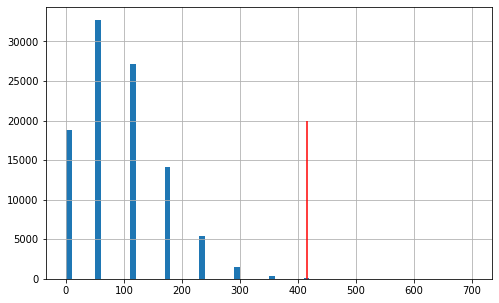
\includegraphics[width=0.7\textwidth]{figures/credit_var_zcb.png}
\caption{Distribution of losses in a portfolio made of twenty zero coupon bonds. The distribution is discrete since all the ZCB have the same face value and recovery rate. The red line indicates the Credit VaR.}
\label{fig:credit_var}
\end{figure}

\subsection{Credit VaR and One Factor Copula Model}
Consider a portfolio made of similar assets. As an approximation assume that the probability of default is the same for each counter-party and that the correlation between each pair is the same and equal to $\rho$. Under these assumption the One Factor Copula model can be used to describe the default correlations (see Eq.~\ref{eq:gaussian_one_factor_copula}

\begin{equation}
\mathcal{Q}_M(T) = \Phi\Big(\cfrac{\Phi^{-1}[Q(T)]-M\sqrt{\rho}}{\sqrt{1-\rho}}\Big)
\label{eq:conditional_default_prob}
\end{equation}
where $\Phi$ is the cumulative distribution function of the standard normal.

If there are $n$ counter-parties with the same default probability $\mathcal{Q}_M(T)$ the percentage of defaults at time $T$ is $\mathcal{Q}_M$ itself ($\textrm{\% of defaults} = \textrm{n\_defaults}/n = n\cdot \mathcal{Q}_M/n$). Hence Eq.~\ref{eq:conditional_default_prob} gives the percentage of defaults by time $T$ given $M$. 

Since $M$ is distributed according to a standard normal we can be $X\%$ certain that its value will be \emph{greater} than $\hat{m} = \Phi^{-1}(1-X)=-\Phi^{-1}(X)$, where the equality holds due to the symmetry of the Gaussian distribution (see Figure~\ref{fig:certain_for_X}).

\begin{figure}[htb]
	\centering
	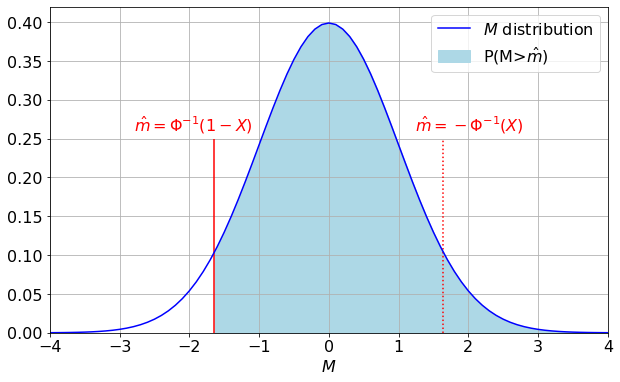
\includegraphics[width=0.7\textwidth]{figures/certain_for_X}
	\caption{$X\%$ probability to get an higher value a threshold for a normally distributed random variable.}
	\label{fig:certain_for_X}
\end{figure} 

Once the time $T$ as been chosen the only random variable appearing in the conditional default probability expression of Eq.~\ref{eq:conditional_default_prob} is $M$, therefore we can be $X\%$ certain that the percentage of defaults over $T$ years on a large portfolio will be \textbf{less} than $V(X,T)$ where
\[
V(X,T)= \Phi\Big(\cfrac{\Phi^{-1}[Q(T)]-\hat{m}\sqrt{\rho}}{\sqrt{1-\rho}}\Big) = \Phi\Big(\cfrac{\Phi^{-1}[Q(T)]+\Phi^{-1}(X)\sqrt{\rho}}{\sqrt{1-\rho}}\Big)
\]
When the confidence level is $X\%$ and the time horizon is $T$, a rough estimate of the Credit VaR is therefore $P(1-R)V(X,T)$, where $P$ is the size of the portfolio and $R$ is the recovery rate.

Suppose that a bank has a total of \euro{100} million of retail exposures. The 1-year probability of default averages to 2\% and the recovery rate averages to 60\%. The copula correlation parameter is estimated as 0.1.

\begin{ipython}
from scipy.stats import norm
from math import sqrt

X = 0.999
rho = 0.1
R = 0.6
Q = 0.02
exposure = 100e6
num = norm.ppf(Q) + sqrt(rho)*norm.ppf(X)
den = sqrt(1-rho)
V = norm.cdf(num/den)
cr_var = exposure*V*(1-R)

print ("Cr-VaR: {:.0f}".format(round(cr_var, -4)))
\end{ipython}
\begin{ioutput}
Cr-VaR: 5130000
\end{ioutput}
\noindent
The 1-year 99.9\% Credit VaR is therefore \euro{5.13} million.

\subsection{CreditMetrics}
Another popular approach to compute Credti VaR is \emph{CreditMetrics}. It involves estimating a probability distribution of credit losses by carrying out Monte Carlo simulations of the counter-party credit rating changes.

Imagine we would like to determine the probability distribution of losses over 1-year period. On each simulation, we are going to determine the credit rating of each counter-party using the estimated probability of migration between one rate to another (or to default). Since the portfolio value depends on its asset ratings we can determine the eventual losses. 

As an example consider Table~\ref{tab:credit_ratings}, it shows the percentage probability of a bond moving from one category to another during a 1-year period.

\begin{table}[htb]
	\centering
	\begin{tabular}{|l|c|c|c|c|c|c|c|c|}
	\hline
	Initial rating & AAA & AA & A & BBB & BB & B & CCC & default \\
	\hline
	\hline
	AAA & 90.81 & 8.33 & 0.68 & 0.06 & 0.08 & 0.02 & 0.01& 0.01 \\ 
	\hline
	AA & 0.70 & 90.65 & 7.79 & 0.64 & 0.06 & 0.13 & 0.02 & 0.01 \\ 
	\hline
	A & 0.09 & 2.27 & 91.05 & 5.52 & 0.74 & 0.26 & 0.01 & 0.06 \\ 
	\hline
	BBB & 0.02 & 0.33 & 5.95 & 85.93 & 5.30 & 1.17 & 1.12 & 0.18 \\
	\hline
	BB & 0.03 & 0.14 & 0.67 & 7.73 & 80.53 & 8.84 & 1.00 & 1.06 \\
	\hline
	B & 0.01 & 0.11 & 0.24 & 0.43 & 6.48 & 83.46 & 4.07 & 5.20 \\
	\hline
	CCC & 0.21 & 0 & 0.22 & 1.30 & 2.38 & 11.24 & 64.86 & 19.79 \\		
	\hline
\end{tabular}
\caption{Example of table with transition probabilities (in percent) between different credit rating categories.}
\label{tab:credit_ratings}
\end{table}

For a correct implementation of this technique credit rate changes cannot be assumed independent, hence a copula approach could be implemented.
Another possibility is the application of Markov chains~\ref{sec:markov_chain}, with the transition matrix which can be deduced by numbers as in Table~\ref{tab:credit_ratings}.

In fact the main difficulty in this application is precisely the determination of the transition matrix. These probabilities could be estimated by analysing historical data from credit rating agencies, such as Standard\&Poor, Moody’s and Fitch. But this could lead to unreliable numbers in case the future does not develop as smoothly as in the past. It can therefore be more reliable to base the estimates on a combination of empirical data and more subjective, qualitative data such as opinions from experts. This is because the market view is a mixture of beliefs determined by both historical ratings and a more extreme view of the ratings. 

Another problem with deciding the transition matrix is that maybe it is not appropriate to use a \emph{homogeneous} Markov chain to model credit risk over time. In this kind of chain the transition matrix is considered constant, but it is clearly a crude approximation of reality which doesn't capture the time-varying behaviour of the default risk. A non-homogeneous model could be more realistic, but on the other hand more complicated to use. 

%As an example suppose to simulate rating change of a portfolio of nine bonds with various ratings over 1-year period. The correlation between them is 0.2.
%
%\begin{codebox}
%\begin{Verbatim}[commandchars=\\\{\}]
%\PY{k+kn}{from} \PY{n+nn}{scipy}\PY{n+nn}{.}\PY{n+nn}{stats} \PY{k}{import} \PY{n}{multivariate\PYZus{}normal}\PY{p}{,} \PY{n}{norm}
%\PY{k+kn}{import} \PY{n+nn}{numpy}
%		
%\PY{c+c1}{\PYZsh{} AAA, AA, A, BBB, BB, B, CCC, Def}
%\PY{n}{table} \PY{o}{=} \PY{p}{[}\PY{p}{[}\PY{l+m+mf}{90.81}\PY{p}{,} \PY{l+m+mf}{8.33}\PY{p}{,} \PY{l+m+mf}{0.68}\PY{p}{,} \PY{l+m+mf}{0.06}\PY{p}{,} \PY{l+m+mf}{0.08}\PY{p}{,} \PY{l+m+mf}{0.02}\PY{p}{,} \PY{l+m+mf}{0.01}\PY{p}{,} \PY{l+m+mf}{0.01}\PY{p}{]}\PY{p}{,}
%         \PY{p}{[}\PY{l+m+mf}{0.70}\PY{p}{,} \PY{l+m+mf}{90.65}\PY{p}{,} \PY{l+m+mf}{7.79}\PY{p}{,} \PY{l+m+mf}{0.64}\PY{p}{,} \PY{l+m+mf}{0.06}\PY{p}{,} \PY{l+m+mf}{0.13}\PY{p}{,} \PY{l+m+mf}{0.02}\PY{p}{,} \PY{l+m+mf}{0.01}\PY{p}{]}\PY{p}{,}
%         \PY{p}{[}\PY{l+m+mf}{0.09}\PY{p}{,} \PY{l+m+mf}{2.27}\PY{p}{,} \PY{l+m+mf}{91.05}\PY{p}{,} \PY{l+m+mf}{5.52}\PY{p}{,} \PY{l+m+mf}{0.74}\PY{p}{,} \PY{l+m+mf}{0.26}\PY{p}{,} \PY{l+m+mf}{0.01}\PY{p}{,} \PY{l+m+mf}{0.06}\PY{p}{]}\PY{p}{,}
%         \PY{p}{[}\PY{l+m+mf}{0.02}\PY{p}{,} \PY{l+m+mf}{0.33}\PY{p}{,} \PY{l+m+mf}{5.95}\PY{p}{,} \PY{l+m+mf}{85.93}\PY{p}{,} \PY{l+m+mf}{5.30}\PY{p}{,} \PY{l+m+mf}{1.17}\PY{p}{,} \PY{l+m+mf}{1.12}\PY{p}{,} \PY{l+m+mf}{0.18}\PY{p}{]}\PY{p}{,}
%         \PY{p}{[}\PY{l+m+mf}{0.03}\PY{p}{,} \PY{l+m+mf}{0.14}\PY{p}{,} \PY{l+m+mf}{0.67}\PY{p}{,} \PY{l+m+mf}{7.73}\PY{p}{,} \PY{l+m+mf}{80.53}\PY{p}{,} \PY{l+m+mf}{8.84}\PY{p}{,} \PY{l+m+mf}{1.00}\PY{p}{,} \PY{l+m+mf}{1.06}\PY{p}{]}\PY{p}{,}
%         \PY{p}{[}\PY{l+m+mf}{0.01}\PY{p}{,} \PY{l+m+mf}{0.11}\PY{p}{,} \PY{l+m+mf}{0.24}\PY{p}{,} \PY{l+m+mf}{0.43}\PY{p}{,} \PY{l+m+mf}{6.48}\PY{p}{,} \PY{l+m+mf}{83.46}\PY{p}{,} \PY{l+m+mf}{4.07}\PY{p}{,} \PY{l+m+mf}{5.20}\PY{p}{]}\PY{p}{,}
%         \PY{p}{[}\PY{l+m+mf}{0.21}\PY{p}{,} \PY{l+m+mi}{0}\PY{p}{,} \PY{l+m+mf}{0.22}\PY{p}{,} \PY{l+m+mf}{1.30}\PY{p}{,} \PY{l+m+mf}{2.38}\PY{p}{,} \PY{l+m+mf}{11.24}\PY{p}{,} \PY{l+m+mf}{64.86}\PY{p}{,} \PY{l+m+mf}{19.79}\PY{p}{]}\PY{p}{]}
%				
%\PY{n}{t} \PY{o}{=} \PY{n}{numpy}\PY{o}{.}\PY{n}{array}\PY{p}{(}\PY{n}{table}\PY{p}{)}
%\PY{n}{table\PYZus{}gauss} \PY{o}{=} \PY{n}{norm}\PY{o}{.}\PY{n}{ppf}\PY{p}{(}\PY{n}{np}\PY{o}{.}\PY{n}{cumsum}\PY{p}{(}\PY{n}{t}\PY{o}{/}\PY{l+m+mf}{100.}\PY{p}{,} \PY{n}{axis}\PY{o}{=}\PY{l+m+mi}{1}\PY{p}{)}\PY{p}{)}
%\PY{n}{table\PYZus{}gauss}\PY{p}{[}\PY{p}{:}\PY{p}{,} \PY{o}{\PYZhy{}}\PY{l+m+mi}{1}\PY{p}{]} \PY{o}{=} \PY{n}{np}\PY{o}{.}\PY{n}{inf}
%		
%\PY{n}{N} \PY{o}{=} \PY{p}{[}\PY{l+m+mi}{100}\PY{p}{,} \PY{l+m+mi}{95}\PY{p}{,} \PY{l+m+mi}{92}\PY{p}{,} \PY{l+m+mi}{85}\PY{p}{,} \PY{l+m+mi}{80}\PY{p}{,} \PY{l+m+mi}{70}\PY{p}{,} \PY{l+m+mi}{60}\PY{p}{]}
%\PY{n}{portfolio} \PY{o}{=} \PY{p}{[}\PY{l+m+mi}{2}\PY{p}{,} \PY{l+m+mi}{3}\PY{p}{,} \PY{l+m+mi}{3}\PY{p}{,} \PY{l+m+mi}{4}\PY{p}{,} \PY{l+m+mi}{5}\PY{p}{,} \PY{l+m+mi}{6}\PY{p}{,} \PY{l+m+mi}{3}\PY{p}{,} \PY{l+m+mi}{4}\PY{p}{,} \PY{l+m+mi}{2}\PY{p}{]}
%\PY{n}{R} \PY{o}{=} \PY{l+m+mf}{0.4}
%		
%\PY{n}{p0} \PY{o}{=} \PY{l+m+mi}{0}
%\PY{k}{for} \PY{n}{i} \PY{o+ow}{in} \PY{n}{portfolio}\PY{p}{:}
%    \PY{n}{p0} \PY{o}{+}\PY{o}{=} \PY{n}{N}\PY{p}{[}\PY{n}{i}\PY{p}{]}
%		
%\PY{n}{numpy}\PY{o}{.}\PY{n}{random}\PY{o}{.}\PY{n}{seed}\PY{p}{(}\PY{l+m+mi}{1}\PY{p}{)}
%\PY{n}{mvnorm} \PY{o}{=} \PY{n}{multivariate\PYZus{}normal}\PY{p}{(}\PY{n}{mean}\PY{o}{=}\PY{p}{[}\PY{l+m+mi}{0} \PY{k}{for} \PY{n}{\PYZus{}} \PY{o+ow}{in} \PY{n+nb}{range}\PY{p}{(}\PY{l+m+mi}{9}\PY{p}{)}\PY{p}{]}\PY{p}{,}
%          \PY{n}{cov}\PY{o}{=}\PY{p}{[}\PY{p}{[}\PY{l+m+mi}{1}\PY{p}{,} \PY{l+m+mf}{0.2}\PY{p}{,} \PY{l+m+mf}{0.2}\PY{p}{,} \PY{l+m+mf}{0.2}\PY{p}{,} \PY{l+m+mf}{0.2}\PY{p}{,} \PY{l+m+mf}{0.2}\PY{p}{,} \PY{l+m+mf}{0.2}\PY{p}{,} \PY{l+m+mf}{0.2}\PY{p}{,} \PY{l+m+mf}{0.2}\PY{p}{]}\PY{p}{,}
%          \PY{p}{[}\PY{l+m+mf}{0.2}\PY{p}{,} \PY{l+m+mi}{1}\PY{p}{,} \PY{l+m+mf}{0.2}\PY{p}{,} \PY{l+m+mf}{0.2}\PY{p}{,} \PY{l+m+mf}{0.2}\PY{p}{,} \PY{l+m+mf}{0.2}\PY{p}{,} \PY{l+m+mf}{0.2}\PY{p}{,} \PY{l+m+mf}{0.2}\PY{p}{,} \PY{l+m+mf}{0.2}\PY{p}{]}\PY{p}{,}
%          \PY{p}{[}\PY{l+m+mf}{0.2}\PY{p}{,} \PY{l+m+mf}{0.2}\PY{p}{,} \PY{l+m+mi}{1}\PY{p}{,} \PY{l+m+mf}{0.2}\PY{p}{,} \PY{l+m+mf}{0.2}\PY{p}{,} \PY{l+m+mf}{0.2}\PY{p}{,} \PY{l+m+mf}{0.2}\PY{p}{,} \PY{l+m+mf}{0.2}\PY{p}{,} \PY{l+m+mf}{0.2}\PY{p}{]}\PY{p}{,}
%          \PY{p}{[}\PY{l+m+mf}{0.2}\PY{p}{,} \PY{l+m+mf}{0.2}\PY{p}{,} \PY{l+m+mf}{0.2}\PY{p}{,} \PY{l+m+mi}{1}\PY{p}{,} \PY{l+m+mf}{0.2}\PY{p}{,} \PY{l+m+mf}{0.2}\PY{p}{,} \PY{l+m+mf}{0.2}\PY{p}{,} \PY{l+m+mf}{0.2}\PY{p}{,} \PY{l+m+mf}{0.2}\PY{p}{]}\PY{p}{,}
%          \PY{p}{[}\PY{l+m+mf}{0.2}\PY{p}{,} \PY{l+m+mf}{0.2}\PY{p}{,} \PY{l+m+mf}{0.2}\PY{p}{,} \PY{l+m+mf}{0.2}\PY{p}{,} \PY{l+m+mi}{1}\PY{p}{,} \PY{l+m+mf}{0.2}\PY{p}{,} \PY{l+m+mf}{0.2}\PY{p}{,} \PY{l+m+mf}{0.2}\PY{p}{,} \PY{l+m+mf}{0.2}\PY{p}{]}\PY{p}{,}
%          \PY{p}{[}\PY{l+m+mf}{0.2}\PY{p}{,} \PY{l+m+mf}{0.2}\PY{p}{,} \PY{l+m+mf}{0.2}\PY{p}{,} \PY{l+m+mf}{0.2}\PY{p}{,} \PY{l+m+mf}{0.2}\PY{p}{,} \PY{l+m+mi}{1}\PY{p}{,} \PY{l+m+mf}{0.2}\PY{p}{,} \PY{l+m+mf}{0.2}\PY{p}{,} \PY{l+m+mf}{0.2}\PY{p}{]}\PY{p}{,}
%          \PY{p}{[}\PY{l+m+mf}{0.2}\PY{p}{,} \PY{l+m+mf}{0.2}\PY{p}{,} \PY{l+m+mf}{0.2}\PY{p}{,} \PY{l+m+mf}{0.2}\PY{p}{,} \PY{l+m+mf}{0.2}\PY{p}{,} \PY{l+m+mf}{0.2}\PY{p}{,} \PY{l+m+mi}{1}\PY{p}{,} \PY{l+m+mf}{0.2}\PY{p}{,} \PY{l+m+mf}{0.2}\PY{p}{]}\PY{p}{,}
%          \PY{p}{[}\PY{l+m+mf}{0.2}\PY{p}{,} \PY{l+m+mf}{0.2}\PY{p}{,} \PY{l+m+mf}{0.2}\PY{p}{,} \PY{l+m+mf}{0.2}\PY{p}{,} \PY{l+m+mf}{0.2}\PY{p}{,} \PY{l+m+mf}{0.2}\PY{p}{,} \PY{l+m+mf}{0.2}\PY{p}{,} \PY{l+m+mi}{1}\PY{p}{,} \PY{l+m+mf}{0.2}\PY{p}{]}\PY{p}{,}
%          \PY{p}{[}\PY{l+m+mf}{0.2}\PY{p}{,} \PY{l+m+mf}{0.2}\PY{p}{,} \PY{l+m+mf}{0.2}\PY{p}{,} \PY{l+m+mf}{0.2}\PY{p}{,} \PY{l+m+mf}{0.2}\PY{p}{,} \PY{l+m+mf}{0.2}\PY{p}{,} \PY{l+m+mf}{0.2}\PY{p}{,} \PY{l+m+mf}{0.2}\PY{p}{,} \PY{l+m+mi}{1}\PY{p}{]}\PY{p}{]}\PY{p}{)}
%		
%\PY{n}{trials} \PY{o}{=} \PY{l+m+mi}{1000000}
%\PY{n}{x\PYZus{}prob} \PY{o}{=} \PY{n}{mvnorm}\PY{o}{.}\PY{n}{rvs}\PY{p}{(}\PY{n}{size}\PY{o}{=}\PY{n}{trials}\PY{p}{)}
%		
%\PY{n}{dp} \PY{o}{=} \PY{p}{[}\PY{p}{]}
%\PY{k}{for} \PY{n}{x} \PY{o+ow}{in} \PY{n}{x\PYZus{}prob}\PY{p}{:}
%    \PY{n}{p} \PY{o}{=} \PY{l+m+mi}{0}
%    \PY{k}{for} \PY{n}{j} \PY{o+ow}{in} \PY{n+nb}{range}\PY{p}{(}\PY{n+nb}{len}\PY{p}{(}\PY{n}{portfolio}\PY{p}{)}\PY{p}{)}\PY{p}{:}
%        \PY{n}{ip} \PY{o}{=} \PY{l+m+mi}{0}
%        \PY{k}{while} \PY{n}{x}\PY{p}{[}\PY{n}{j}\PY{p}{]} \PY{o}{\PYZgt{}} \PY{n}{table\PYZus{}gauss}\PY{p}{[}\PY{n}{portfolio}\PY{p}{[}\PY{n}{j}\PY{p}{]}\PY{p}{,} \PY{n}{ip}\PY{p}{]}\PY{p}{:}
%            \PY{n}{ip} \PY{o}{+}\PY{o}{=} \PY{l+m+mi}{1}
%            \PY{k}{if} \PY{n}{ip} \PY{o}{==} \PY{l+m+mi}{7}\PY{p}{:}
%                \PY{n}{p} \PY{o}{+}\PY{o}{=} \PY{n}{N}\PY{p}{[}\PY{n}{portfolio}\PY{p}{[}\PY{n}{j}\PY{p}{]}\PY{p}{]}\PY{o}{*}\PY{p}{(}\PY{l+m+mi}{1}\PY{o}{\PYZhy{}}\PY{n}{R}\PY{p}{)}
%            \PY{k}{else}\PY{p}{:}
%                \PY{n}{p} \PY{o}{+}\PY{o}{=} \PY{n}{N}\PY{p}{[}\PY{n}{ip}\PY{p}{]}
%	
%        \PY{n}{r} \PY{o}{=} \PY{n+nb}{max}\PY{p}{(}\PY{l+m+mi}{0}\PY{p}{,} \PY{o}{\PYZhy{}}\PY{p}{(}\PY{n}{p} \PY{o}{\PYZhy{}} \PY{n}{p0}\PY{p}{)}\PY{p}{)}
%        \PY{k}{if} \PY{n}{r} \PY{o}{!=} \PY{l+m+mi}{0}\PY{p}{:}
%            \PY{n}{dp}\PY{o}{.}\PY{n}{append}\PY{p}{(}\PY{n}{r}\PY{p}{)}
%		
%\PY{n}{crvar} \PY{o}{=} \PY{n}{numpy}\PY{o}{.}\PY{n}{percentile}\PY{p}{(}\PY{n}{dp}\PY{p}{,} \PY{p}{[}\PY{l+m+mf}{99.9}\PY{p}{]}\PY{p}{)}
%\PY{n+nb}{print} \PY{p}{(}\PY{n}{crvar}\PY{p}{)}
%
%[124.]
%\end{Verbatim}
%\end{codebox}
%
%\begin{figure}[htb]
%	\centering
%	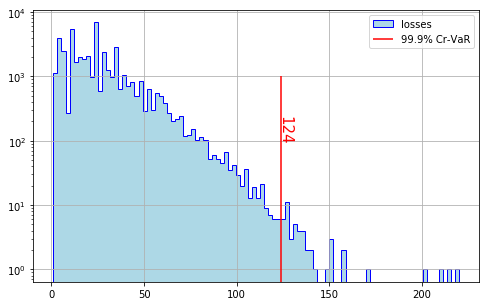
\includegraphics[width=0.7\textwidth]{figures/credit_metrics.png}
%	\caption{Distribution of the losses estimated from simulation of credit rating changes within 1 year. The red line shows the 99.9\% Cr-VaR.}
%\end{figure}

\section{Credit Valuation Adjustment}
\label{credit-valuation-adjustment}

Suppose you have a portfolio of derivatives with a counter-party. If it defaults and the present value of the portfolio at default is positive to the surviving party, then the gain is only given by a recovery fraction of the portfolio value. If however the present value is negative to the surviving party, it has to pay it in full to the liquidators of the defaulted entity.

This behaviour creates and asymmetry which can be corrected by defining the deal value as the value without counter-party risk minus a positive adjustment, called \emph{Credit Valuation Adjustment} (CVA).

The CVA can be expressed in the following way:

\begin{equation}
\text{CVA} = (1-R) \int_0^T D(t) \cdot \textrm{EE}(t) dQ(t)
\label{eq:cva}
\end{equation}
where $T$ is the latest maturity in the portfolio, $D$ is the discount factor, EE is the expected exposure or \(\mathbb{E}[\text{max(0, NPV}_\text{portfolio})]\), and $dQ$ is the probability of default between $t$ and $t+dt$.

For an easier computation it is natural to discretize the above integral and use a time grid going from 0 to the portfolio maturity:

\begin{equation}
\text{CVA} = (1-R) \sum_i^n D(t_i) \cdot \mathrm{EE}(t_i) Q(t_{i-1}, t_i)
\label{eq:cva_discrete}
\end{equation}

It is important to note the difference between Credit VaR and CVA. While the former measures the risk of losses faced due to the possible default of some counter-party, the latter measures the pricing component of this risk, i.e. the price adjustment of a product due to this risk.

\subsection{Debit Valuation Adjustment}

The adjustment seen from the point of view of our counter-party is positive, and is called Debit Valuation Adjustment, DVA. It is positive because the early default of the client itself would imply a discount on the client payment obligations, and this means a gain. So the client marks a positive adjustment over the risk free price by adding the positive amount called DVA. 

When both parties have the possibility to default, they consistently include both defaults into the valuation. Hence
every party needs to include its own default besides the default of the counter-party into the valuation. So they will mark a positive CVA to be subtracted and a positive DVA to be added to the default risk free price of the deal. The CVA of one party will be the DVA of the other one and vice versa.

\[
\textrm{price}=\textrm{default risk free price + DVA - CVA}
\]
Now, since
\[
\textrm{default risk free price(A)} = - \textrm{default risk free price(A)}
\]
\[
\textrm{DVA(A)} = \textrm{CVA(B)}
\]
\[
\textrm{DVA(B)} = \textrm{CVA(A)}
\]
we get that eventually
\[
\textrm{price(A)} = -\textrm{price(B)}
\]
so that both parties agree on the price, or, we could say, there is money conservation.

\subsection{CVA Computation}

The computation of the CVA is easily carried on with Monte Carlo simulation. First simulate the development of your portfolio (its NPV) at each time point for each MC scenario. Then calculate the CVA using Eq.~\ref{eq:cva} or its discrete form in Eq.~\ref{eq:cva_discrete}. Finally average the CVA of all the scenarios to get its estimate.

In case of zero coupon bonds the computation of the CVA can be further simplified. Indeed in this case the exposure of the investor is equal to the face value of the bond, so it is enough to loop through each day from the observation date to the bond maturity and compute the CVA using Eq.~\ref{eq:cva_discrete}.

Imagine a 3-years zero coupon bond with a face value of $FV=$~\euro{100}. The bond issuer has the following default probabilities 10\%, 20\% and 30\% for 1, 2 and 3 years respectively and the recovery rate is 40\%. The risk free rate is instead 3\%. 

To compute the CVA we need to first define a discount curve and the issuer credit curve. Then we perform a daily loop to sum up all the contributions to the CVA and finally set the price of the bond to the default-risk-free price minus the CVA.

\begin{ipython}
from dateutil.relativedelta import relativedelta
from finmarkets import DiscountCurve, CreditCurve
import math

T = 3
r = 0.03
R = 0.4
FV = 100
obs_date = date.today()
pillars = [obs_date+relativedelta(years=i) for i in range(T+1)]
dfs = [math.exp(-r*i) for i in range(T+1)]
dc = DiscountCurve(obs_date, pillars, dfs)
S = [1, 0.9, 0.8, 0.7]
cc = CreditCurve(pillars, S)
PV = FV * math.exp(-r*i)
cva = 0
d = obs_date
while d <= pillars[-1]:
    cva += dc.df(d)*(cc.ndp(d) - cc.ndp(d+relativedelta(days=1)))
    d += relativedelta(days=1)
cva *= (1-R) * FV

print ("CVA: {:.2f}".format(cva))
print ("Bond Price: {:.2f}".format(PV - cva))
\end{ipython}
\begin{ioutput}
CVA: 17.21
Bond Price: 74.18
\end{ioutput}

\section*{Exercises}
\begin{question}
Given the historical series of three stock prices in the file \href{https://raw.githubusercontent.com/matteosan1/finance_course/master/input_files/historical.csv}{historical.csv} compute the 1-day 95\% VaR and the corresponding Expected shortfall for a portfolio consisting of 40 FOX shares, 35 ABC shares and 25 CBS shares. 

\noindent\textbf{Hint:} when simulating the historical scenarios take care of possible NaN values in the series.
\end{question}

\cprotEnv\begin{solution}
\begin{ipython}
import pandas as pd
import numpy as np

df = pd.read_csv("historical.csv", index_col='date')
w = np.array([0.4, 0.25, 0.35])

df['P'] = df[['FOX', 'CBS', 'ABC']].dot(w)
df = df.pct_change()
df.dropna(inplace=True)
print (df.head())
\end{ipython}
\begin{ioutput}
                 FOX       CBS       ABC         P
date                                              
2018-03-26  0.013858 -0.012607  0.011189  0.006395
2018-03-23 -0.030891 -0.046818 -0.010830 -0.024072
2018-03-22  0.020592  0.020093  0.011543  0.015722
2018-03-21  0.003317  0.012137  0.052941  0.031266
2018-03-20 -0.003306 -0.011991 -0.003464 -0.005276
\end{ioutput}
\begin{ipython}
from numpy.random import seed, choice
from numpy import percentile
from finmarkets import var_discrete, es_discrete
 
var = var_discrete(df, 0.95, 'P')
es = es_discrete(df, 0.95, 'P')

print (f"VaR: {var:.4f}")
print (f"ES: {es:.4f}")
\end{ipython}
\begin{ioutput}
VaR: 0.0173
ES: 0.0232
\end{ioutput}
\begin{figure}[htbp]
\centering
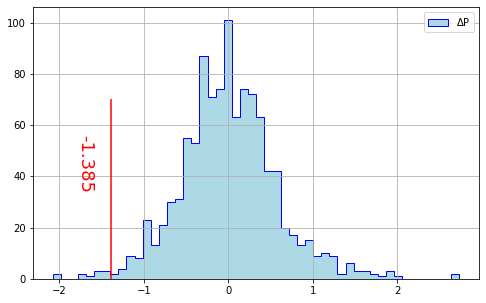
\includegraphics[width=0.7\linewidth]{figures/hist_var_ex}
\end{figure}
\end{solution}

\begin{question}
You have a 3-years call with strike 110 EUR. The underlying initial price is 105 EUR with a volatility of 0.15. The risk-free rate is 0.03 flat.
Compute the CVA of the contract assuming a recovery rate of 40\% and default probabilities for the underlying of 10\%, 20\% and 30\% for first, second and third year respectively.
\end{question}

\cprotEnv\begin{solution}
Below are shown ten realizations of the underlying price.

\begin{figure}[htbp]
\centering
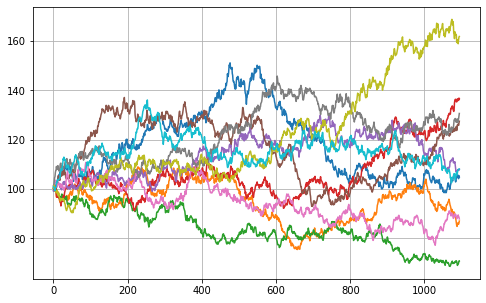
\includegraphics[width=0.7\linewidth]{figures/underlying_simulation}
\end{figure}

This implementation is not optimized in terms of speed, indeed it takes about 2 minutes to run 500 simulations.
A different approach, fully exploiting \texttt{numpy.array}s, could allow to shrink the execution time by a factor of 200.

\begin{ipython}
from datetime import date
from dateutil.relativedelta import relativedelta
from finmarkets import CreditCurve, call
from scipy.stats import norm
import numpy as np
import time

K = 110
sigma = 0.15
r = 0.03
T = 3
steps = 365*T
dt = 1/365
R = 0.4
Q = [0.9, 0.8, 0.7]
S0 = 105

obs_date = date.today()
dates = [obs_date + relativedelta(years=i+1) for i in range(T)]
cc = CreditCurve(obs_date, dates, Q)
t1 = time.time()
scenarios = 500
St = np.zeros(shape=(steps, scenarios))
St[0, :] = S0
ndps = np.zeros(shape=(steps,))
for i in range(1, steps):
    St[i, :] = St[i-1, :] * np.exp((r - 0.5 * sigma**2) * dt \
        + sigma* np.sqrt(dt) * norm.rvs(size=scenarios))
    ndps[i] = cc.ndp(obs_date+relativedelta(days=i-1)) - \
        cc.ndp(obs_date+relativedelta(days=i))

ts = [f"{t}y" for t in np.arange(T-dt, 0, -dt)]
cvas = np.zeros(shape=(steps, scenarios))
for s in range(scenarios):
    for j in range(len(ts)):
        cvas[j, s] = call(St[j, s], K, r, sigma, ts[j])*(1-R)*ndps[j]
cvas = np.sum(cvas, axis=0)
print (np.mean(cvas))
print (time.time() - t1)
\end{ipython}
\begin{ioutput}
2.464147656202549
129.0265169143676
\end{ioutput}
\end{solution}

\begin{question}
\label{ex:credit_var}
Consider a 1-years call with strike 110 EUR. The underlying initial price is 100 EUR with a volatility of 0.50. The risk-free rate is 0.03 flat. Compute the 99.9\% Credit VaR assuming a recovery rate of 40\% and default probabilities for the underlying of 30\% within next year.
\end{question}

\cprotEnv\begin{solution}

In order to increase the number of simulations the implemented code fully uses \texttt{numpy.array}.

\begin{ipython}
import numpy as np
from datetime import date
from dateutil.relativedelta import relativedelta
from finmarkets import CreditCurve
from scipy.stats import norm


K = 110
sigma = 0.50
r = 0.03
T = 1
steps = 365*T
dt = 1/365
R = 0.4
S0 = 100

obs_date = date.today()
cc = CreditCurve(obs_date, [obs_date + relativedelta(years=1)], [0.7])
scenarios = 10000
St = np.zeros(shape=(steps, scenarios))
St[0, :] = S0
ndps = np.zeros(shape=(steps,))
for i in range(1, steps):
    St[i, :] = St[i-1, :] * np.exp((r - 0.5 * sigma**2) * dt \
                                   + sigma* np.sqrt(dt) * norm.rvs(size=scenarios))
    ndps[i] = cc.ndp(obs_date+relativedelta(days=i)) - \
        cc.ndp(obs_date+relativedelta(days=i+1))

ts = [f"{t}y" for t in np.arange(T-dt, 0, -dt)]
EE = np.zeros(shape=(steps, scenarios))
for s in range(scenarios):
    EE[1:, s] = call(St[:-1, s], K, r, sigma, ts)*(1-R)*ndps[1:]
EE = np.sum(EE, axis=0)
print (f"Credit VaR: {np.percentile(EE, 99.9):.3f}")
\end{ipython}
\begin{ioutput}
Credit VaR: 26.281
\end{ioutput}

\begin{figure}[htbp]
\centering
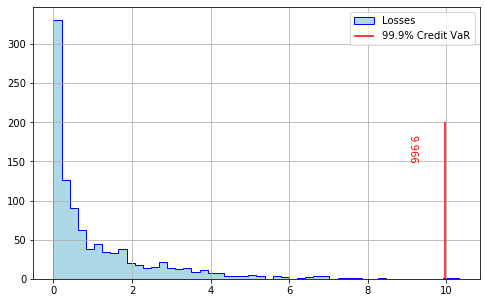
\includegraphics[width=0.7\linewidth]{figures/cr_var_ex}
\caption{Loss distribution to estimate Credit VaR measure of Ex.~\ref{ex:credit_var}.}
\end{figure}
\end{solution}







\begin{thebibliography}{9}
\bibitem{bib:var} J. C. Hull, \emph{Options, Futures and Other Derivatives, 7th Ed.}, Value at Risk (Ch. 20), Pearson Prentice Hall, 2009
\bibitem{bib:credit_var} J. C. Hull, \emph{Options, Futures and Other Derivatives, 7th Ed.}, Credit Risk (Ch. 22), Pearson Prentice Hall, 2009
\bibitem{bib:creditmetrics}RiskMetrics Group, \href{https://www.msci.com/documents/10199/93396227-d449-4229-9143-24a94dab122f}{\emph{CreditMetrics}}, J.P. Morgan \& Co., 2007, [Online]
\bibitem{bib:cva} D. Brigo, \emph{Counterparty Risk FAQ: Credit VaR, PFE, CVA, DVA, Closeout, Netting, Collateral, Re-hypothecation, WWR, Basel, Funding, CCDS and Margin Lending}, arXiv: 1111.1331, 2011
\end{thebibliography}